\newlength{\textAreaHeight}
\setlength{\textAreaHeight}{0.75\paperheight}

\section{Definition und Architektur}

\begin{frame}
    \frametitle{Data Warehouse: Definition}
    
    \begin{notebox}
    \hl{Data Warehouse} :=
    \begin{itemize}
    \item \hl{dauerhafte}
    \item \hl{integrierte} Sammlung von Daten
    \item aus \hl{unterschiedlichen} Quellen
    \item zum \hl{Zweck der Analyse} bzw. Entscheidungsunterstützung
    \end{itemize}
    \end{notebox}
    
    \end{frame}

    
\begin{frame}[shrink]
    \frametitle{Data Warehouse: Charakteristika}

    \begin{itemize}
    \item \hl{Fachorientierung (subject-oriented):}
    \begin{itemize}
    %\item Zweck des Systems ist nicht Erfüllung einer Aufgabe (z.B. Personaldatenverwaltung), sondern Modellierung eines spezifischen Anwendungsziels
    \item Zweck ist Unterstützung bereichsübergreifender Auswertungsmöglichkeiten für unterschiedliche Domänen
    \item Zentralisierte Bereitstellung der Daten über Geschäftsobjekte (Themen)
    \end{itemize}
    \item \hl{Integrierte Datenbasis (integrated):}
    \begin{itemize}
    \item Verarbeitung von Daten aus mehreren verschiedenen (internen und externen) Datenquellen (z.B. operationalen DB oder Web)
    \end{itemize}
    \item \hl{Nicht-flüchtige Datenbasis (non-volatile):}
    \begin{itemize}
    \item stabile, persistente Datenbasis
    \item Daten im DW werden i. A. nicht mehr entfernt oder geändert
    \end{itemize}
    \item \hl{Zeitbezogene Daten (time-variant):}
    \begin{itemize}
    \item Vergleich der Daten über Zeit möglich (Zeitreihenanalyse)
    \item Speicherung über längeren Zeitraum
    \end{itemize}
    \end{itemize}

    \end{frame}

    %--------------------------------------------------------------

    \begin{frame}
        \frametitle{DW-Architektur: Komponenten}
    
        \begin{itemize}
        \item Datenquellen: Herkunftsort der Daten
        \item Datenbereinigungsbereich: temporäre Datenbank für Transformation
        \item Data Warehouse: physische Datenbank für Analyse
        \item Repository: Datenbank mit Metadaten
        \item ETL-Prozess: Extraktion, Transformation, Laden = Datenvorbereitung
        \end{itemize}
    
        \begin{center}
        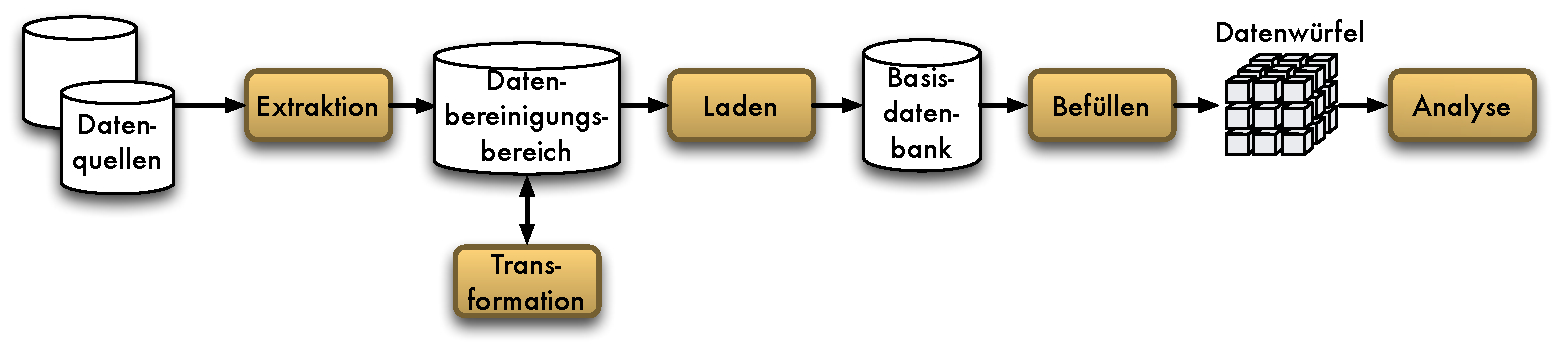
\includegraphics[width=.99\textwidth]{fig6/Referenzarchitektur-1.pdf}
        \end{center}
    
        \end{frame}
        %--------------------------------------------------------------
    
    \begin{frame}[c]
        \frametitle{Beispiel einer Anfrage}
    
        \begin{beamercolorbox}[sep=4pt,colsep*=5pt,shadow=true,rounded=false]{sqlexample}%
        \begin{quote}
            Welche \hl{Umsätze} sind in den \hl{Jahren} 2009 und 2010 in den
                \hl{Warensegmenten} Bier und Rotwein in den
                \hl{Bundesländern} Sachsen-Anhalt und Thüringen angefallen?
        \end{quote}
        \end{beamercolorbox}
    
        \end{frame}
    

    \section{Datenmodellierung}

    \frame{
      \frametitle{Überblick}
      \tableofcontents[currentsection,hidesubsections,firstsection=24]
    }


    \begin{frame}

        \frametitle{Grundbegriffe}
        \begin{itemize}
            \item Dimensionen
            \item Fakten / Kennzahlen
        \end{itemize}
        \begin{center}
        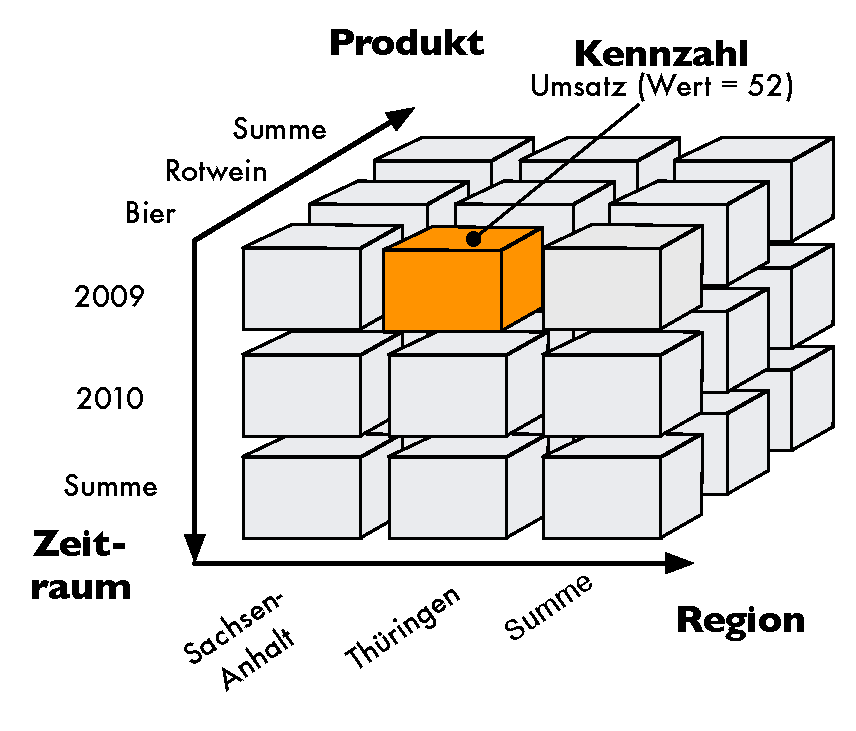
\includegraphics[height=0.8\textAreaHeight]{fig6/Wuerfel.pdf}
        \end{center}

        \end{frame}

        \begin{frame}

        \frametitle{Motivation}
        \begin{itemize}
        \item Datenmodell ausgerichtet auf Unterstützung der Analyse
        \item Datenanalyse im Entscheidungsprozess
          \begin{itemize}
          \item Betriebswirtschaftliche Kennzahlen  stehen im Mittelpunkt\\ $\to$ \hl{Fakten}

            $\bullet$ Gewinn, $\bullet$ Umsatz, $\bullet$ Kosten, $\bullet$ etc.
          \item Betrachtung der Kennzahlen aus unterschiedlichen Perspektiven\\ $\to$ \hl{Dimensionen}

            $\bullet$  Zeit, $\bullet$  Raum, $\bullet$  Sache
          \item Unterteilung der Auswertedimensionen möglich\\ $\to$ \hl{Hierarchien} oder
            \hl{Konsolidierungsebenen}

          $\bullet$  Jahr, $\bullet$  Quartal, $\bullet$  Monat
        \end{itemize}
        \end{itemize}
        \end{frame}

        %%%%%%%%%%%%%%%%%%%%%%%%%%%%%%%%%%%%%%%%%%%%%%%%%%%%%%%%%%%%%%%%%%%%%%%%
        \begin{frame}

        \frametitle{Verfügbare Informationen}

        \begin{itemize}
        \item Qualifizierend
        \begin{itemize}
        \item Repräsentiert durch "`Kategorienattribute"'
        \item Daten zur Nutzung als Navigationsraster ("`Drill-Pfade"')
        \item Modelliert als Begriffshierarchien im Rahmen von Dimensionen
        \end{itemize}
        \item Quantifizierend
        \begin{itemize}
        \item Bilden Gegenstand der Auswertung \\
        ("`Summenattribute"' oder andere arithmetische Operationen)
        \item Zellen eines Würfels, mit Dimensionen als Kanten
        \end{itemize}
        \end{itemize}

        \end{frame}

        %%%%%%%%%%%%%%%%%%%%%%%%

        \begin{frame}

        \frametitle{Dimensionen}
        \begin{itemize}
        \item Dimension:
        \begin{itemize}
        \item Beschreibt mögliche Sicht auf assoziierte Kennzahlen
        \item Endliche Menge von $n$ ($n \geq 2$) Dimensionselementen
          (Hierarchieobjekten), die eine semantische Beziehung aufweisen
        \item Dienen der orthogonalen Strukturierung des Datenraums
        \end{itemize}
        \item Beispiele:
        \begin{itemize}
            \item Produkt,
            \item Filialstruktur,
            \item Geschäftsjahr
        \end{itemize}
        \end{itemize}

        \end{frame}

        %%%%%%%%%%%%%%%%%%%%%%%%
        \begin{frame}

        \frametitle{Hierarchien in Dimensionen}
        \begin{itemize}
        \item Dimensionselemente:
        \begin{itemize}
        \item Knoten einer Klassifikationshierarchie
        \item Klassifikationsstufe beschreibt Verdichtungsgrad
        \item Darstellung von Dimensionen über Klassifikationsschema (Schema
          von Klassifikationshierarchien)
        \end{itemize}
        \item Formen:
        \begin{itemize}
        \item Einfache Hierarchien
        \item Parallele Hierarchien
        \end{itemize}
        \end{itemize}
        \end{frame}

        %%%%%%%%%%%%%%%%%%%%%%%%
        \begin{frame}

        \frametitle{Einfache Hierarchie}
        \begin{itemize}
        \item Höhere Hierarchieebene enthält die aggregierten Werte genau
          einer niedrigeren Hierarchiestufe
        \item Oberster Knoten: $Top$
          \begin{itemize}
          \item
            Enthält Verdichtung auf einen einzelnen Wert für die Dimension
          \end{itemize}
        \end{itemize}

        \begin{center}
        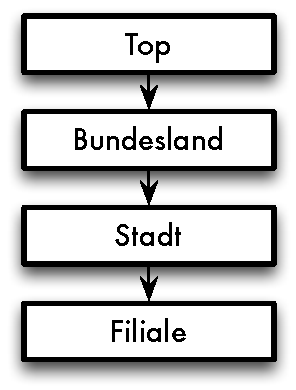
\includegraphics[scale=.46]{fig6/Einfache-Hierarchien.pdf}
        \end{center}
        \end{frame}

        %%%%%%%%%%%%%%%%%%%%%%%%
        \begin{frame}

        \frametitle{Parallele Hierarchie}

        \begin{itemize}
        \item Innerhalb einer Dimension sind mehrere unabhängige Arten der
          Gruppierung möglich
        \item Keine hierarchische Beziehung zwischen parallelen Zweigen
        \item Parallelhierarchie: $\bullet$ Pfad im Klassifikationsschema $\bullet$ Konsolidierungspfad

        \end{itemize}

        \begin{center}
        %\hspace{5cm}
        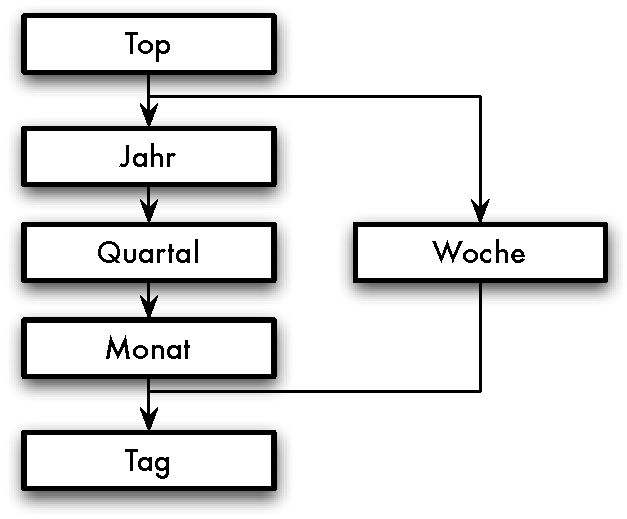
\includegraphics[height=0.46\textAreaHeight]{fig6/Parallele-Hierarchien.pdf}
        \end{center}

        \end{frame}

        %%%%%%%%%%%%%%%%%%%%%%%%


        \begin{frame}

        \frametitle{Kategorienattribute}
        \begin{itemize}
        \item Inhaltliche Verfeinerung durch unterschiedliche Rollen:
        \item Primärattribut
          \begin{itemize}
          \item Kategorienattribut, das alle anderen Attribute einer Dimension
            bestimmt
          \item Definiert maximale Feinheit
          \item Beispiel: "`Auftragsposition"'
        \end{itemize}
        \item Klassifikationsattribut
          \begin{itemize}
          \item Element der Menge, die mehrstufige Kategorisierung
            (Klassifikationshierarchie) bilden
          \item Beispiel: "`Produkt"', "`Produktgruppe"', "`Produktkategorie"'
        \end{itemize}
        \item Dimensionales Attribut
          \begin{itemize}
          \item Element der Menge der Attribute, die vom Primärattribut oder
            einem Klassifikationsattribut bestimmt werden und nur $Top_D$
            bestimmen
          \item Beispiel: "`Regalposition"'
        \end{itemize}
        \end{itemize}

        \end{frame}

        %%%%%%%%%%%%%%%%%%%%%%%%
        \begin{frame}

        \frametitle{Struktur einer Dimension: Beispiel}

        \begin{center}
        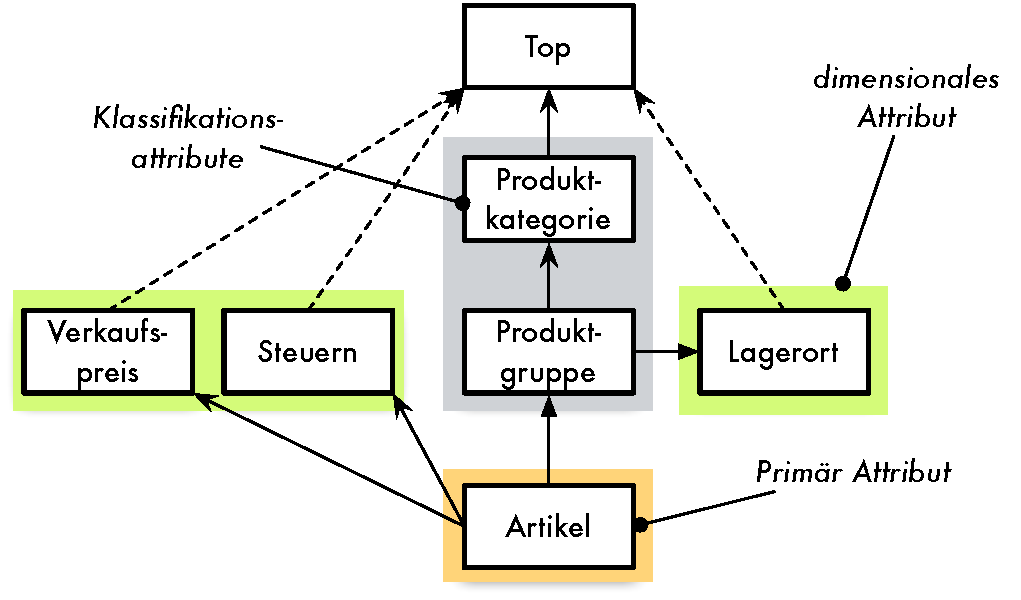
\includegraphics[scale=.6]{fig6/Dimensionsstruktur.pdf}
        \end{center}
        \end{frame}

        %%%%%%%%%%%%%%%%%%%%%%%%
        \begin{frame}

        \frametitle{Kennzahlen}
        \begin{itemize}
        \item Kennzahlen / Fakten (engl. \emph{facts}):
          \begin{itemize}
          \item (Verdichtete) numerische Messgrößen
          \item Beschreiben betriebswirtschaftliche Sachverhalte
          \end{itemize}
        \item \hl{Fakt}: Maßzahl (engl. \emph{measure})
        \item \hl{Kennzahl}:
          \begin{itemize}
          \item Aus Fakten konstruiert (abgeleitete Kennzahl)
          \item Durch Anwendung arithmetischer Operationen
          \end{itemize}
        \item  Beispiele:
          \begin{itemize}
          \item Umsatz, Gewinn, Kosten
          \item Deckungsbeitrag, ROI (Return on Investment)
          \item Fluktuationsquote, Umsatzsteigerung
          \end{itemize}
        \end{itemize}

        \end{frame}

        %%%%%%%%%%%%%%%%%%%%%%%%

        \begin{frame}

          \frametitle{Fakt: Schema}
        %Besteht aus
          \begin{itemize}
          \item Schema wird durch mehrere  Bestandteile spezifiziert
          \item \hl{Granularität} $G = \{ G_1, \dots , G_k \}$
            \begin{itemize}
            \item $G$ ist Teilmenge aller Kategorienattribute aller im Schema
              existierenden Dimensionsschemata $\leadsto$ keine funktionalen Abhängigkeit zwischen Kategorienattributen
                einer Granularität
            \item "`Detailliertheitsgrad"' der Fakten
            \end{itemize}
          \item \hl{Summationstyp} $SumTyp$
          \begin{itemize}
              \item Bestandsgröße STOCK
              \item Stromgröße FLOW
              \item Einheit VALUE-PER-UNIT
            \end{itemize}
          \end{itemize}


        \end{frame}

        %%%%%%%%%%%%%%%%%%%%%%%%

        \begin{frame}

        \frametitle{Kennzahl}
        \begin{itemize}
        \item \hl{Kennzahl} $M$ ist definiert durch
        \begin{itemize}
        \item Granularität $G$
        \item Berechnungsvorschrift $f()$ über Fakten
        \item Summationstyp $SumTyp$
        \end{itemize}
        \item Berechnung über nichtleerer Teilmenge der im Schema
          existierenden Fakten
        \end{itemize}

        \end{frame}

        %%%%%%%%%%%%%%%%%%%%%%%%

        \begin{frame}

        \frametitle{Kennzahl: Bildung von f()}
        \begin{itemize}
        \item Skalarfunktionen
          \begin{itemize}
          \item $+, -, *, /, mod$
          \item Beispiel: $Umsatzsteueranteil = Menge * Preis * Steuersatz$
          \end{itemize}
        \item Aggregatfunktionen
          \begin{itemize}
          \item Funktion $H()$ zur Verdichtung eines Datenbestandes, indem aus
            $n$ Einzelwerten ein Aggregatwert ermittelt wird
        $$ H: 2 ^{dom(X_1) \times \cdots \times  dom(X_n)} \to dom(Y)$$
        \item Bsp.: $SUM(), AVG(), MIN(), MAX(), COUNT()$
        \end{itemize}
        \item Ordnungsbasierte Funktionen
          \begin{itemize}
          \item Definition von Kennzahlen auf Basis zuvor definierter
            Ordnungen
          \item Bsp.: Kumulation, $TOP(n)$, $MEDIAN()$
          \end{itemize}
        \end{itemize}

        \end{frame}

        %%%%%%%%%%%%%%%%%%%%%%%%
        \begin{frame}

        \frametitle{Summationstypen}
        \begin{itemize}
        \item Zuweisung eines \hl{Summationstyps} charakterisiert erlaubte
          Aggregationsoperationen
        \item Stromgröße (FLOW)
          \begin{itemize}
          \item zeitraumbezogen (pro Zeiteinheit)
          \item Beliebig aggregierbar
          \item Beispiel: Bestellmenge eines Artikels pro Tag
          \end{itemize}
        \item Bestandsgröße (STOCK)
          \begin{itemize}
          \item Maß über Zeitraum
          \item Beliebig aggregierbar mit Ausnahme temporaler Dimension
          \item Beispiel: Lagerbestand, Einwohnerzahl
          \end{itemize}
        \item Einheit (VALUE-PER-UNIT - VPU)
          \begin{itemize}
          \item zeitpunktbezogen (zum Zeitpunkt)
          \item Aktuelle Zustände, die nicht summierbar sind
          \item Zulässig nur: $MIN(), MAX(), AVG()$
          \item Beispiele: Preis, Wechselkurs, Steuersatz
        \end{itemize}
        \end{itemize}

        \end{frame}

        %%%%%%%%%%%%%%%%%%%%%%%%
        \begin{frame}

        \frametitle{Summierbarkeit}

        \begin{center}

                \begin{tabular}{|c|c|c|c|c|}
                \hline &	FLOW	& \multicolumn{2}{c|}{STOCK} & 	VPU \\
                \hline  && \multicolumn{2}{c|}{Aggregation	über} &\\
                && \multicolumn{2}{c|}{temporale Dimension?}	& \\
                  \cline{3-4}		&&	nein&	ja&	\\
                \hline	\hline $MIN/MAX$	&$+$	&\multicolumn{2}{c|}{$+$}		&$+$\\
                \hline	$SUM$	&$+$	&$+$&	$-$&	$-$\\
                \hline	$AVG$	&$+$&\multicolumn{2}{c|}{$+$}	&	$+$\\
                \hline	$COUNT$	&$+$	&\multicolumn{2}{c|}{$+$}	&$	+$\\
                \hline
                \end{tabular}
        \end{center}

        \end{frame}

        %%%%%%%%%%%%%%%%%%%%%%%%

\section{Relationale Speicherung}


        \begin{frame}

            \frametitle{Relationale Speicherung}
            \begin{itemize}
            \item Vermeidung des Verlustes anwendungsbezogener Semantik (aus dem
              multidimensionalen Modell, z.B. Klassifikationshierarchien)
            \item Effiziente Übersetzung multidimensionaler Anfragen
            \item Effiziente Verarbeitung der übersetzten Anfragen
            \item Einfache Pflege der entstandenen Relationen (z.B. Laden neuer
              Daten)
            \item Berücksichtigung der Anfragecharakteristik und des Datenvolumens
              von Analyseanwendungen
            \end{itemize}
        
            \end{frame}
        
            %%%%%%%%%%%%%%%%%%%%%%%%%%%%%%%%%%%%%%%%%%%%%%%%%%%%%%%%%%%%%%%%%%%%%%%%
        
            \begin{frame}
        
            \frametitle{Relationale Umsetzung: Faktentabelle}
            \begin{itemize}
            \item Ausgangspunkt: Umsetzung des Datenwürfels ohne
              Klassifikationshierarchien
              \begin{itemize}
              \item Dimensionen, Kennzahlen $\to$ Spalten der Relation
              \item Zelle $\to$ Tupel
              \end{itemize}
            \end{itemize}
        
            \begin{columns}[c]
            \begin{column}{3.5cm}
              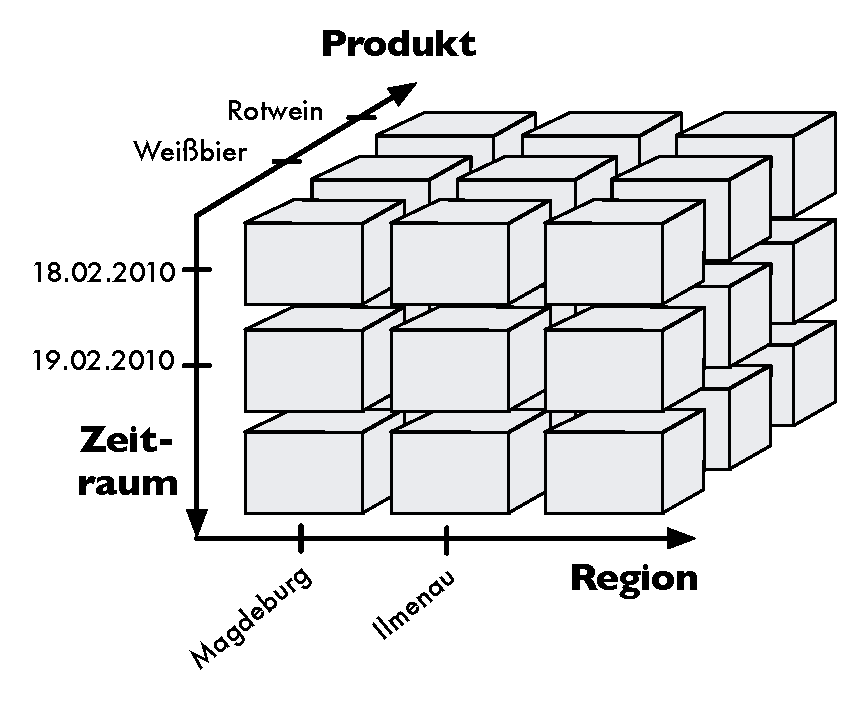
\includegraphics[width = 1.3\textwidth]{fig6/Faktentabelle.pdf}
            \end{column}
            \begin{column}{5cm}
            {\scriptsize
            \begin{tabular}{|l|l|l|c|}
            \hline
            \rowcolor{Gray}  Produkt & Filiale & Tag & Verk. \\
            \hline
            \hline
            Rotwein & Magdeburg & 18.02.10 & 145 \\
            Weißbier & Magdeburg & 18.02.10 & 267 \\
            Rotwein & Ilmenau & 18.02.10 & 70 \\
            \multicolumn{4}{|c|}{\dots}\\
            \hline
            \end{tabular}
            }
            \end{column}
            \end{columns}
            \end{frame}
        
            %%%%%%%%%%%%%%%%%%%%%%%%%%%%%%%%%%%%%%%%%%%%
            \begin{frame}
        
            \frametitle{Snowflake-Schema}
        
            \begin{itemize}
            \item Abbildung von Klassifikationen: eigene Tabelle für jede
              Klassifikationsstufe (z.B. Artikel, Produktgruppe, etc.)
            \item Dimensionstabelle enthält
              \begin{itemize}
              \item ID für Klassifikationsknoten
              \item Beschreibendes Attribut (z.B. Marke, Hersteller, Bezeichnung)
              \item Fremdschlüssel der direkt übergeordneten Klassifikationsstufe
              \end{itemize}
            \item Faktentabelle enthält (neben Kenngrößen):
              \begin{itemize}
              \item Fremdschlüssel der jeweils niedrigsten Klassifikationsstufe
              \item Fremdschlüssel bilden zusammengesetzte Primärschlüssel für
                Faktentabelle
              \end{itemize}
            \end{itemize}
        
            \end{frame}
        
            %%%%%%%%%%%%%%%%%%%%%%%%%%%%%%%%%%%%%%%%%%%%
            \begin{frame}
        
            \frametitle{Snowflake-Schema: Muster}
        
            \begin{center}
              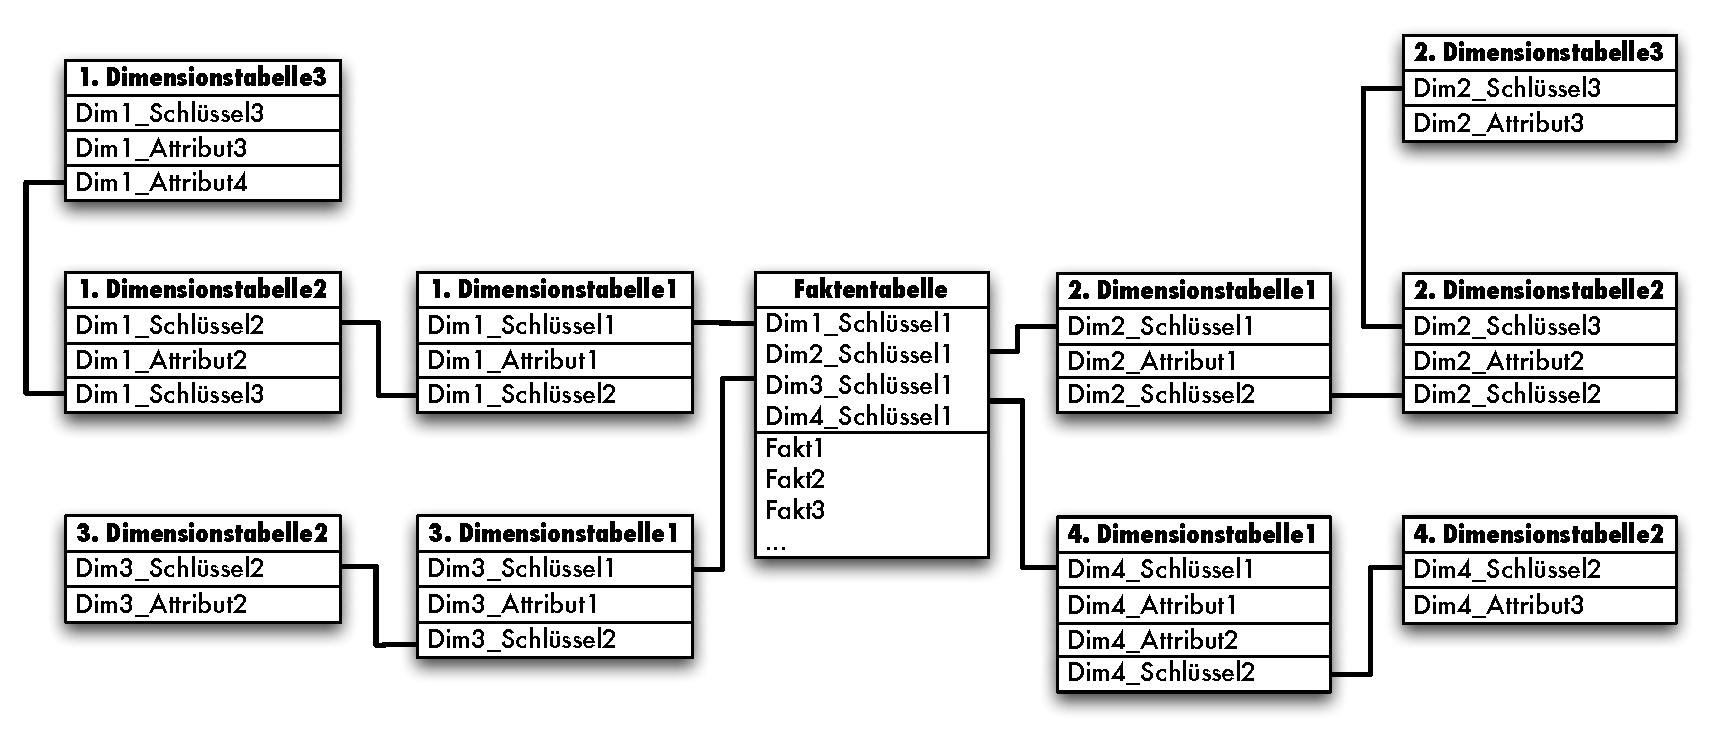
\includegraphics[width=\textwidth]{fig6/Snowflake-Schema.pdf}
            \end{center}
        
            \end{frame}
            %%%%%%%%%%%%%%%%%%%%%%%%%%%%%%%%%%%%%%%%%%%%
            \begin{frame}
        
            \frametitle{Snowflake-Schema: Beispiel}
        
            \begin{center}
              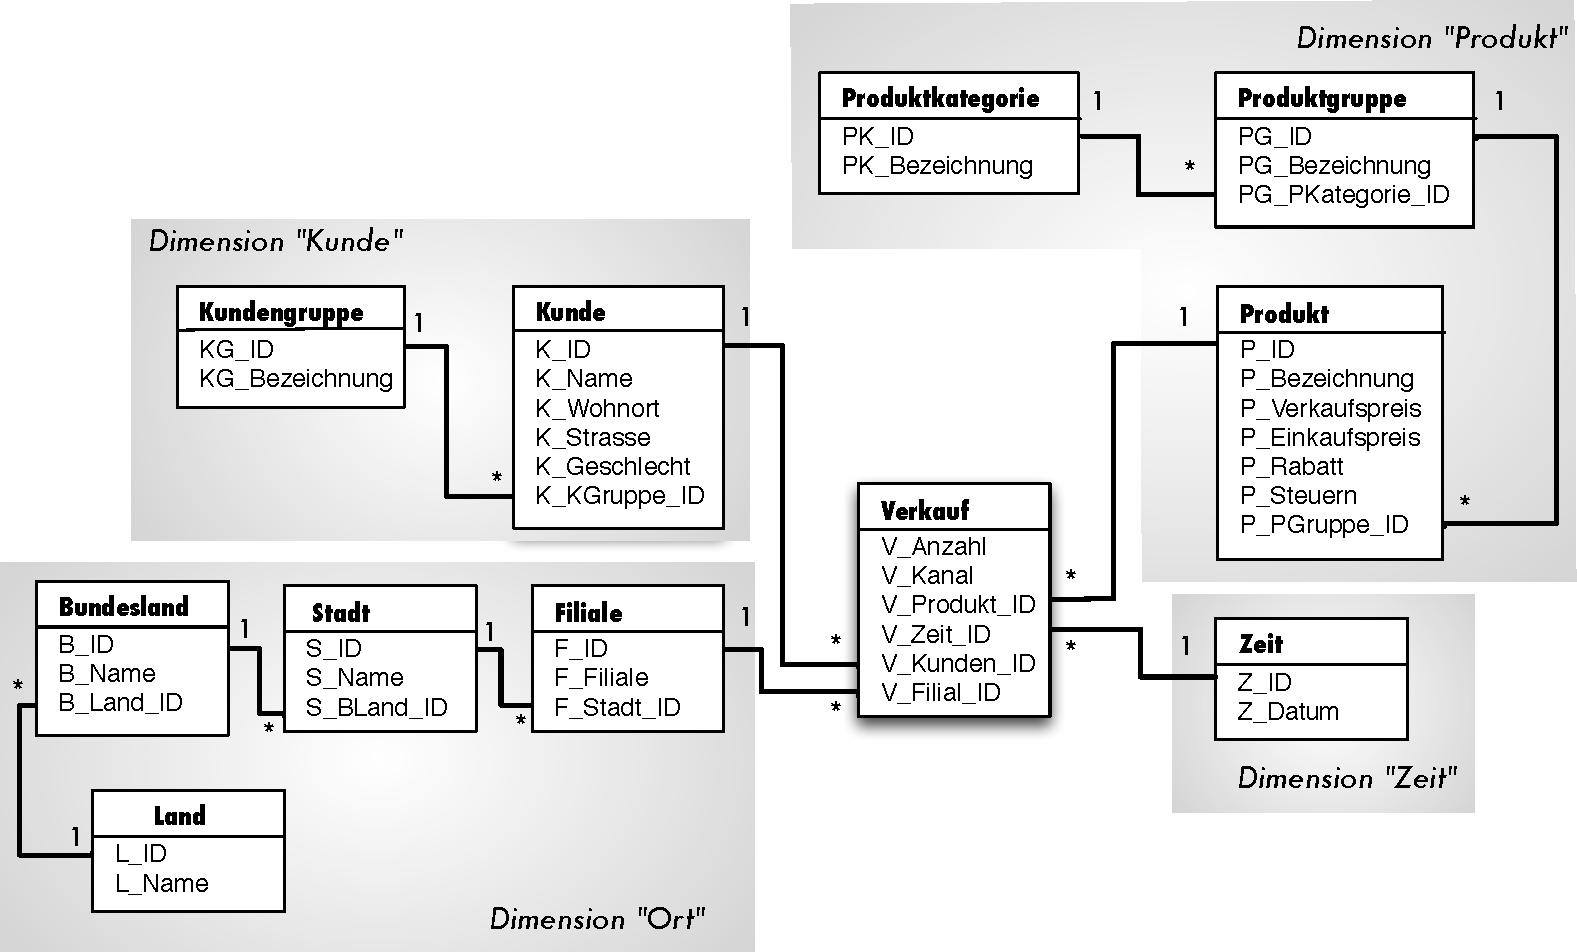
\includegraphics[height=\textAreaHeight,width=\textwidth,keepaspectratio]{fig6/SnowflakeSchema-Buch.pdf}
            \end{center}
        
            \end{frame}
        
            %%%%%%%%%%%%%%%%%%%%%%%%%%%%%%%%%%%%%%%%%%%%
        
            \begin{frame}
        
            \frametitle{Star-Schema}
        
            \begin{itemize}
            \item Snowflake-Schema ist normalisiert: Vermeidung von
              Update-Anomalien $\to$ \hl{3. NF}
              \begin{itemize}
              \item Aber: erfordert Join über mehrere Tabellen!
              \end{itemize}
            \item Star-Schema:
              \begin{itemize}
              \item Denormalisierung der zu einer Dimension gehörenden Tabellen $\to$ \hl{1. NF}
              \item Für jede Dimension genau eine Dimensionstabelle
              \item Redundanzen in der Dimensionstabelle für schnellere
                Anfragebearbeitung
              \item Beispiel: Artikel, Produkt, Produktgruppe etc. als Spalten in
                einer Tabelle Produkt
              \end{itemize}
            \end{itemize}
        
            \end{frame}
        
            %%%%%%%%%%%%%%%%%%%%%%%%%%%%%%%%%%%%%%%%%%%%
        
            \begin{frame}
        
            \frametitle{Star-Schema: Muster}
        
            \begin{center}
              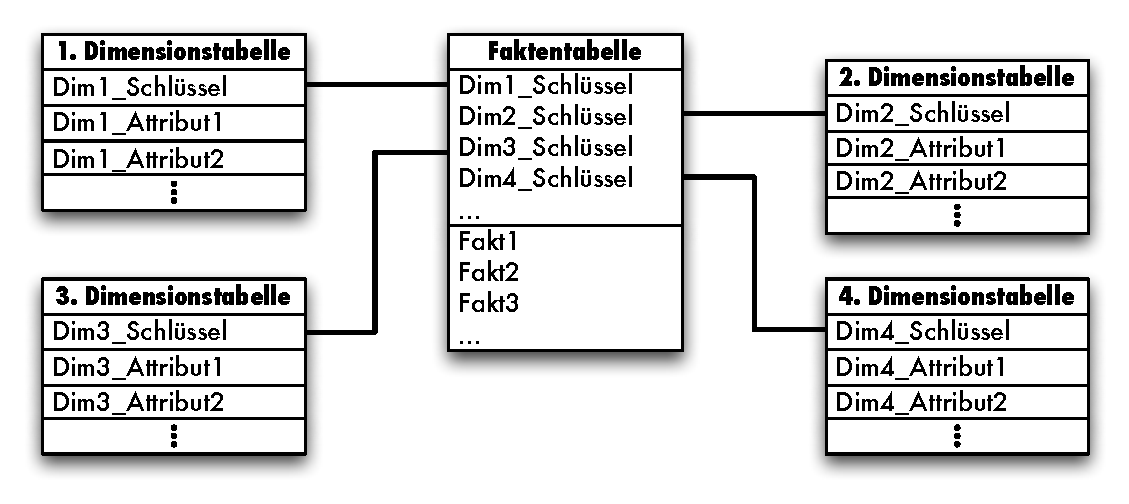
\includegraphics[scale=.6]{fig6/StarSchema.pdf}
            \end{center}
        
            \end{frame}
        
            %%%%%%%%%%%%%%%%%%%%%%%%%%%%%%%%%%%%%%%%%%%%
        
        
            \begin{frame}
        
            \frametitle{Star-Schema: Beispiel}
        
            \begin{center}
              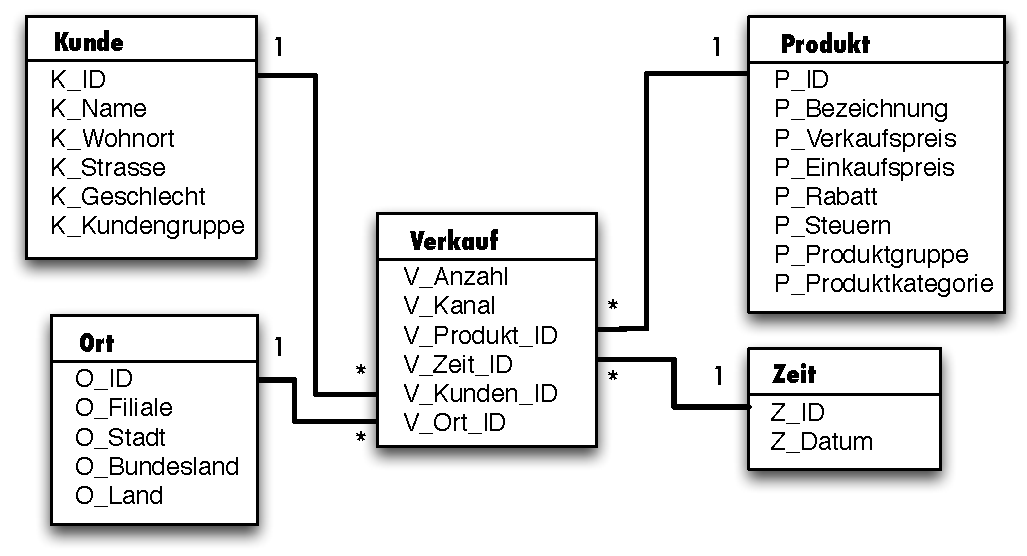
\includegraphics[height=\textAreaHeight,width=\textwidth,keepaspectratio]{fig6/Star-Schema.pdf}
            \end{center}
        
        
            \end{frame}
        
            %%%%%%%%%%%%%%%%%%%%%%%%%%%%%%%%%%%%%%%%%%%%
            \begin{frame}
        
            \frametitle{Star-Schema formal}
        
            \begin{itemize}
            \item Multidimensionales Schema mit $n$ Dimensionen
              \begin{itemize}
              \item Dimensionstabellen $D^1, \dots, D^n$ der Form $D^i(Dim_i\_Key,
                A_{i,1}, \dots, A_{i,{k_i}})$
              \item Faktentabelle $F(Dim_1\_Key, \dots, Dim_n\_Key, f_1, \dots, f_m)$ mit $m$ Fakten
              \end{itemize}
            \item Jeder Teil des kompositen Primärschlüssels der Faktentabelle ist
              Fremdschlüssel zum Primärschlüsselattribut der korrespondierenden
              Dimension
            \end{itemize}
        
            \end{frame}
        
            \begin{frame}
        
                \frametitle{Mischformen}
        
                \begin{itemize}
                \item Abbildung einzelner Dimensionen analog Snowflake-Schema oder
                  Star-Schema
                \item Entscheidungskriterien:
                  \begin{itemize}
                  \item Änderungshäufigkeit der Dimensionen:
                    \begin{itemize}
                    \item Reduzierung des Pflegeaufwandes durch Normalisierung
                      (Snowflake)
                    \end{itemize}
                  \item Anzahl der Klassifikationsstufen einer Dimension:
                    \begin{itemize}
                    \item Mehr Klassifikationsstufen $\to$ größere Redundanz im
                      Star-Schema
                    \end{itemize}
        
                  \item Anzahl der Dimensionselemente:
                    \begin{itemize}
                    \item Einsparung durch Normalisierung bei vielen Elementen einer
                      Dimension auf niedrigster Klassifikationsstufe
                    \end{itemize}
                  \item Materialisierung von Aggregaten:
                    \begin{itemize}
                    \item Performance-Verbesserung durch Normalisierung bei
                      materialisierten Aggregaten für eine Klassifikationsstufe
                    \end{itemize}
                  \end{itemize}
                \end{itemize}
        
                \end{frame}
        
        
                %%%%%%%%%%%%%%%%%%%%%%%%%%%%%%%%%%%%%%%%%%%%
                \begin{frame}
        
                \frametitle{Galaxie-Schema}
        
        
                \begin{itemize}
                \item Star- und Snowflakeschema
                  \begin{itemize}
                  \item Eine Faktentabelle
                  \item Mehrere Kennzahlen nur möglich bei gleichen Dimensionen
                  \end{itemize}
                \item Galaxie-Schema
                  \begin{itemize}
                  \item Mehrere Faktentabellen
                  \item Teilweise mit gleichen Dimensionstabellen verknüpft
                  \item Auch: Multi-Faktentabellen-Schema, Multi-Cube, Hyper-Cube
                  \end{itemize}
                \end{itemize}
        
                \end{frame}
        
                %%%%%%%%%%%%%%%%%%%%%%%%%%%%%%%%%%%%%%%%%%%%
                \begin{frame}
        
                \frametitle{Galaxie-Schema: Muster}
        
                \begin{center}
                  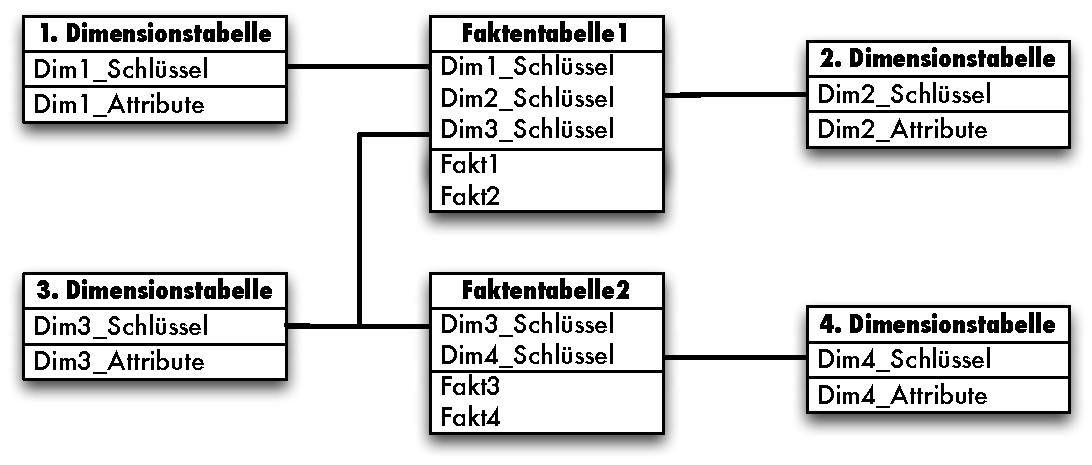
\includegraphics[width=\textwidth]{fig6/Galaxy-Schema.pdf}
                \end{center}
        
                \end{frame}
                %%%%%%%%%%%%%%%%%%%%%%%%%%%%%%%%%%%%%%%%%%%%
        
                \begin{frame}
        
                \frametitle{Galaxie-Schema: Beispiel}
        
                \begin{center}
                  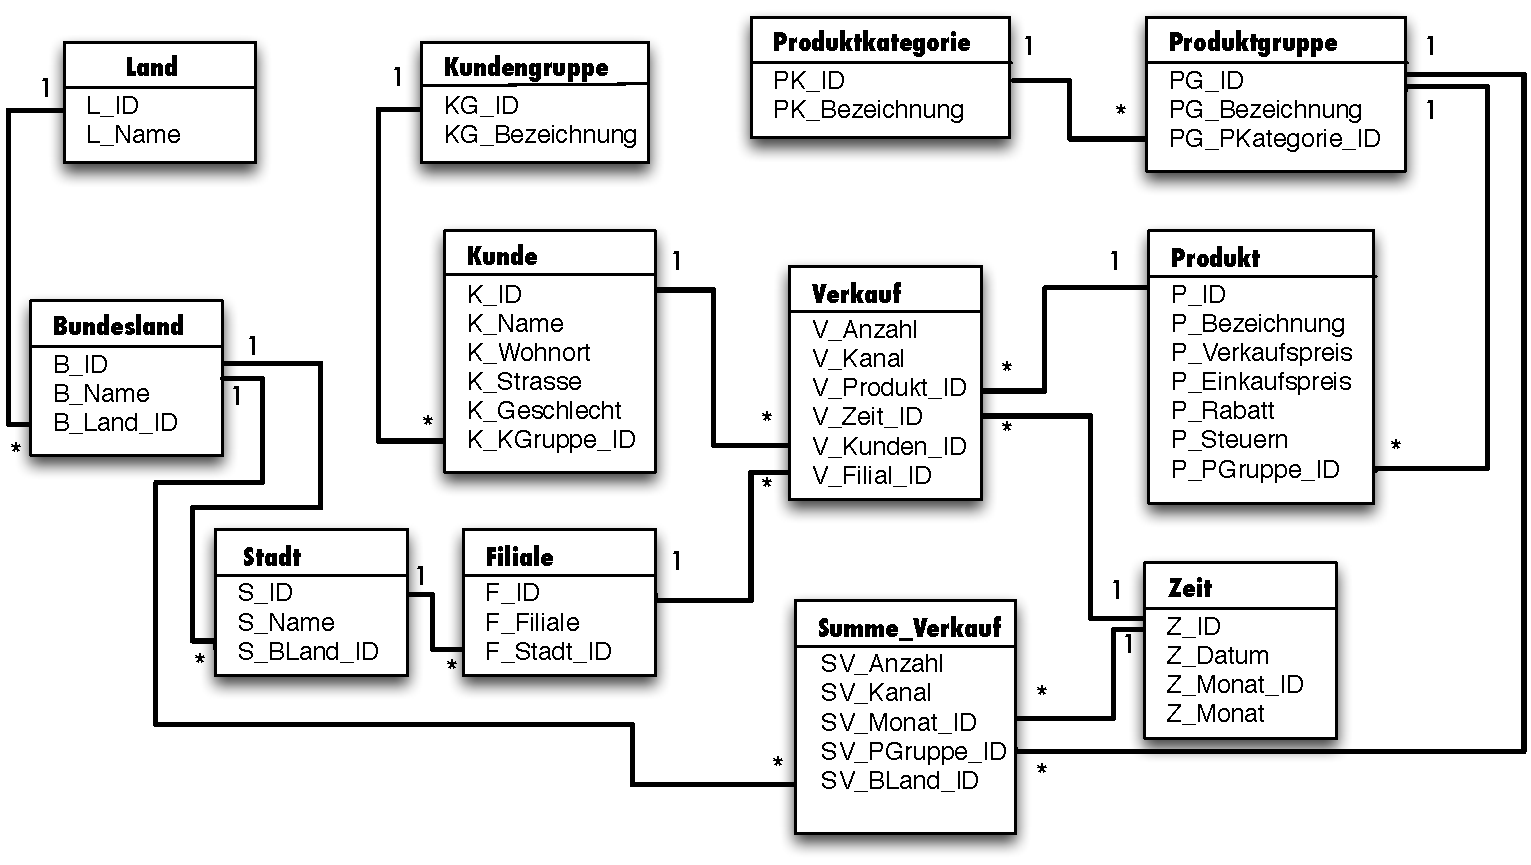
\includegraphics[height=\textAreaHeight,width=\textwidth,keepaspectratio]{fig6/GalaxySchema-Beispiel.pdf}
                \end{center}
        
                \end{frame}
                %%%%%%%%%%%%%%%%%%%%%%%%%%%%%%%%%%%%%%%%%%%%
        
                \begin{frame}
        
                \frametitle{Fact Constellation}
                \begin{itemize}
                \item Speicherung vorberechneter Aggregate in Faktentabelle
                  \begin{itemize}
                  \item Beispiel: Umsatz für Region
                  \item Unterscheidung in Dimensionstabelle über spezielle Attribute
                    (Bsp.: "`Stufe"')
                  \end{itemize}
                \item Alternative: Auslagerung in eigene Faktentabelle
                  \begin{itemize}
                  \item Fact-Constellation-Schema (Spezialfall eines Galaxie-Schemas)
                  \end{itemize}
                \end{itemize}
        
                \end{frame}
        
                %%%%%%%%%%%%%%%%%%%%%%%%%%%%%%%%%%%%%%%%%%%%
        
        
        
                \begin{frame}
        
                \frametitle{Fact Constellation: Beispiel}
        
                \begin{center}
                  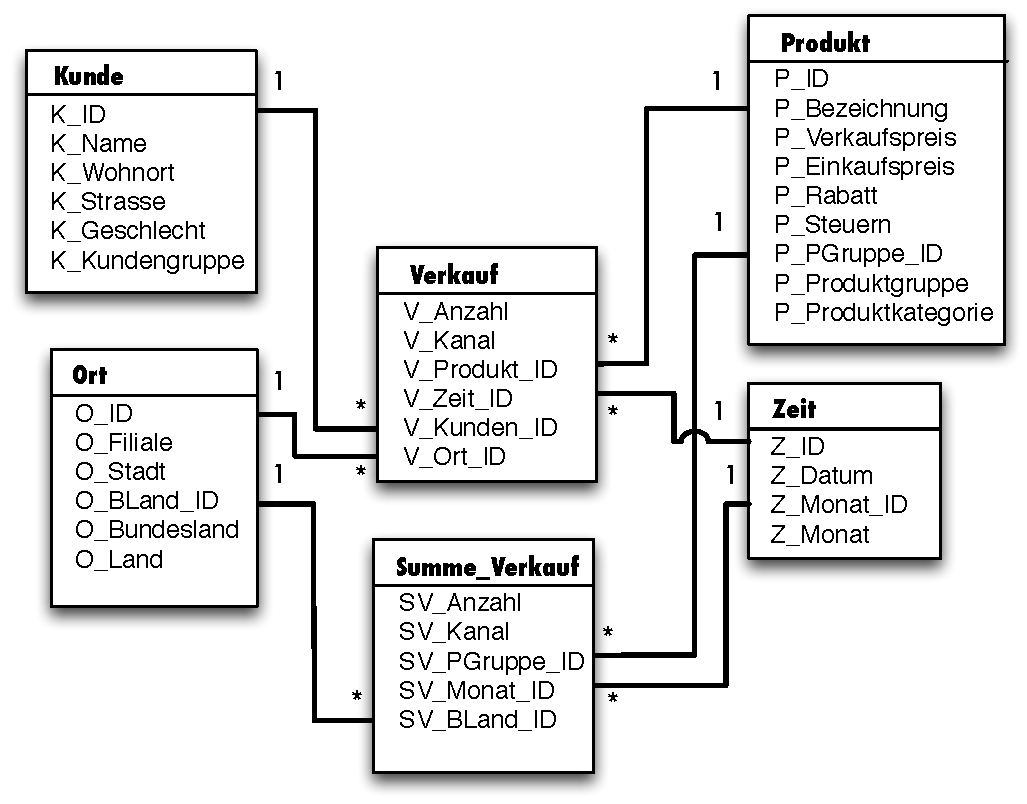
\includegraphics[height=\textAreaHeight]{fig6/Fact-Constellation-Schema.pdf}
                \end{center}
        
        
                \end{frame}
        
        
        \section{OLAP-Operationen zur Datenanalyse}
        
        
        \frame{
          \frametitle{Überblick}
          \tableofcontents[currentsection,hidesubsections,firstsection=24]
        }
        
        \begin{frame}
        
        \frametitle{Operationen zur Datenanalyse}
        \begin{itemize}
        \item OLAP-Operationen auf multidimensionalen Datenstrukturen
        \item Standardoperationen
          \begin{itemize}
          \item Pivotierung
          \item Roll-Up, Drill-Down
          \item Drill-Across
          \item Slice und Dice
          \end{itemize}
        \end{itemize}
        
        
        \end{frame}
        
        %%%%%%%%%%%%%%%%%%%%%%%%
        
        \begin{frame}
        
        \frametitle{Pivotierung / Rotation}
        \begin{itemize}
        \item Drehen des Würfels durch Vertauschen der Dimensionen
        \item Analyse der Daten aus verschiedenen Perspektiven
        \end{itemize}
        
        \begin{center}
        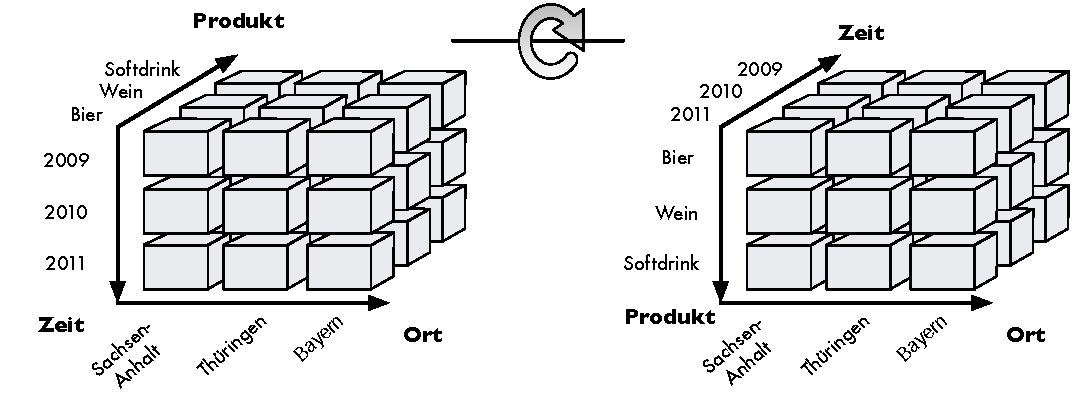
\includegraphics[scale=.6]{fig6/OLAP-Pivot.pdf}
        \end{center}
        \end{frame}
        
        %%%%%%%%%%%%%%%%%%%%%%%%
        
        \begin{frame}
        
        \frametitle{Roll-Up, Drill-Down, Drill-Across}
        \begin{itemize}
        \item \hl{Roll-Up}:
          \begin{itemize}
          \item Erzeugen neuer Informationen durch Aggregierung der Daten
            entlang des Konsolidierungspfades
          \item Dimensionalität bleibt erhalten
          \item Beispiel: Tag $\to$ Monat $\to$ Quartal $\to$ Jahr
          \end{itemize}
        \item \hl{Drill-Down}:
          \begin{itemize}
          \item Komplementär zu Roll-Up
          \item Navigation von aggregierten Daten zu Detail-Daten entlang der
            Klassifikationshierarchie
          \end{itemize}
        \item \hl{Drill-Across}:
          \begin{itemize}
          \item Wechsel von einem Würfel zu einem anderen
          \end{itemize}
        \end{itemize}
        
        
        \end{frame}
        
        %%%%%%%%%%%%%%%%%%%%%%%%
        
        \begin{frame}
        
        \frametitle{Roll-Up und Drill-Down}
        
        \begin{center}
        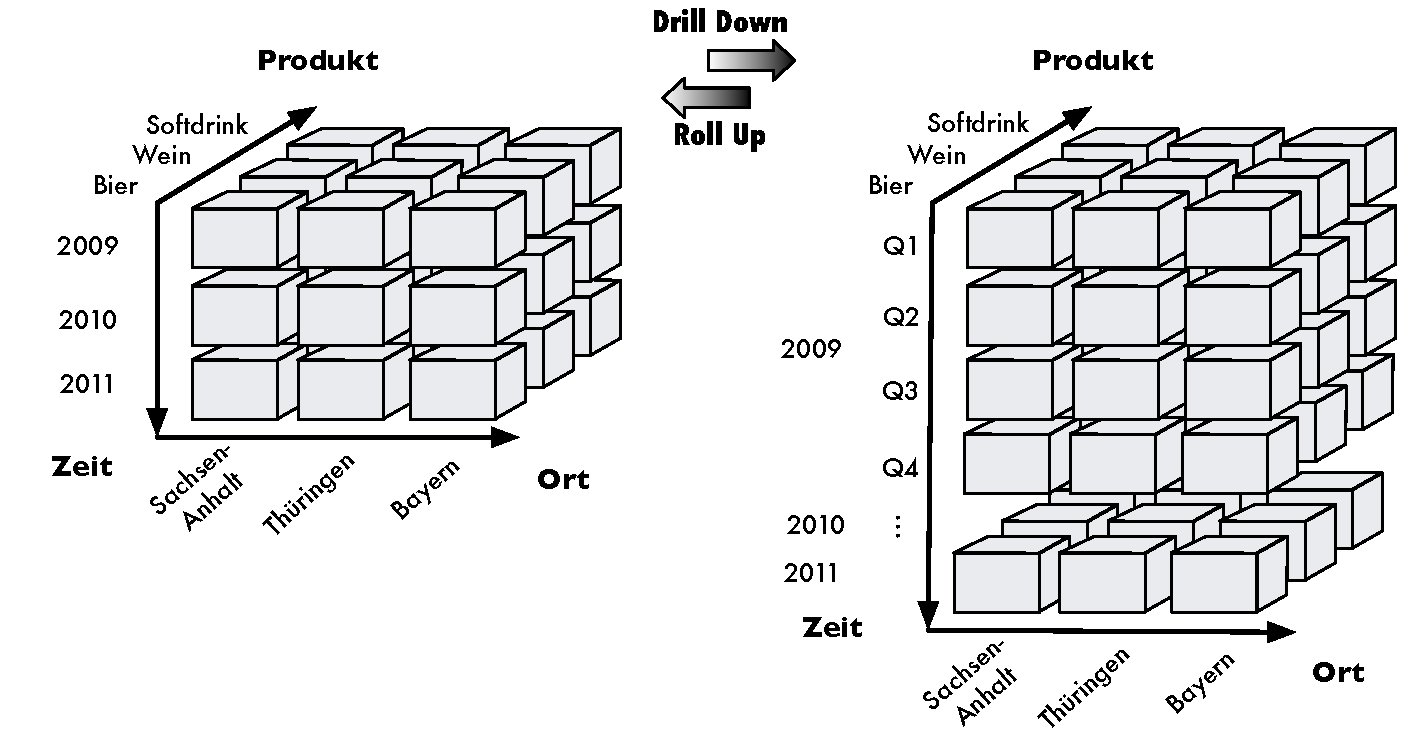
\includegraphics[scale=.46]{fig6/OLAP-DrillDown.pdf}
        \end{center}
        \end{frame}
        
        %%%%%%%%%%%%%%%%%%%%%%%%
        
        
        \begin{frame}
        
        \frametitle{Slice und Dice}
        \begin{itemize}
        \item Erzeugen individueller Sichten
        \item \hl{Slice}:
          \begin{itemize}
          \item Herausschneiden von "`Scheiben"' aus dem Würfel
          \item Verringerung der Dimensionalität durch Konditionierung der Dimensionen
          \item Beispiel: alle Werte des aktuellen Jahres
           \item \emph{Entspricht der relationalen Selektion in den Dimensionen}
          \end{itemize}
        \item \hl{Dice}:
          \begin{itemize}
          \item Herausschneiden einen "`Teilwürfels"'
          \item Erhaltung der Dimensionalität, Veränderung der
            Hierarchieobjekte
          \item Beispiel: die Werte bestimmter Produkte oder Regionen
          \item \emph{Entspricht der relationalen Selektion mehrerer Dimensionen}
        \end{itemize}
        \end{itemize}
        
        \end{frame}
        
        %%%%%%%%%%%%%%%%%%%%%%%%
        
        \begin{frame}
        
        \frametitle{Slice}
        
        \begin{center}
        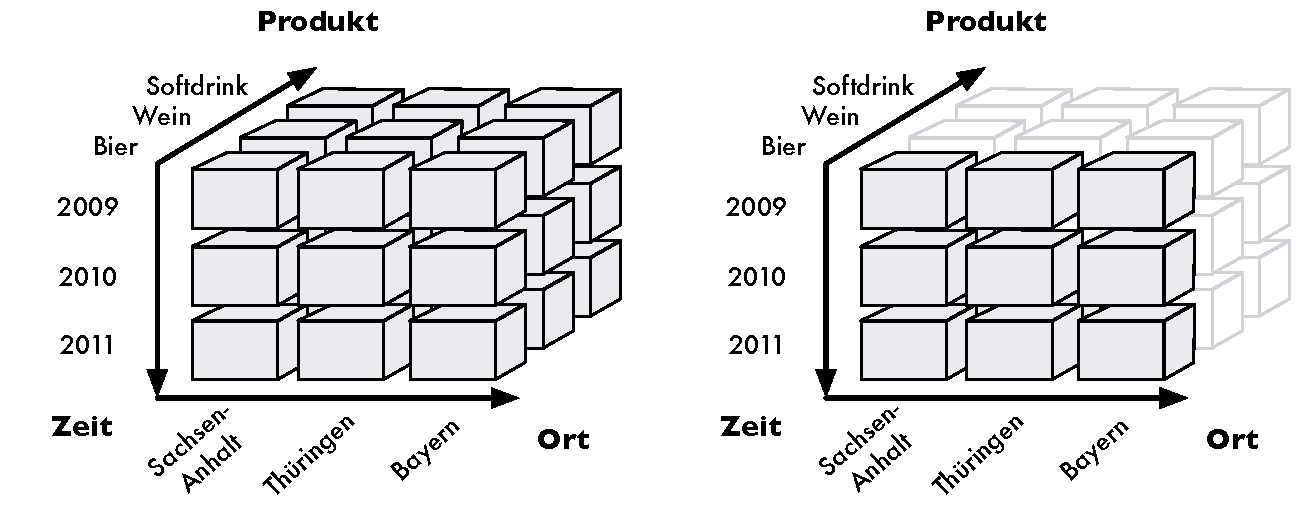
\includegraphics[width=.95\textwidth]{fig6/OLAP-Slice.pdf}
        \end{center}
        
        \end{frame}
        %%%%%%%%%%%%%%%%%%%%%%%%
        
        \begin{frame}
        
        \frametitle{Dice}
        
        \begin{center}
        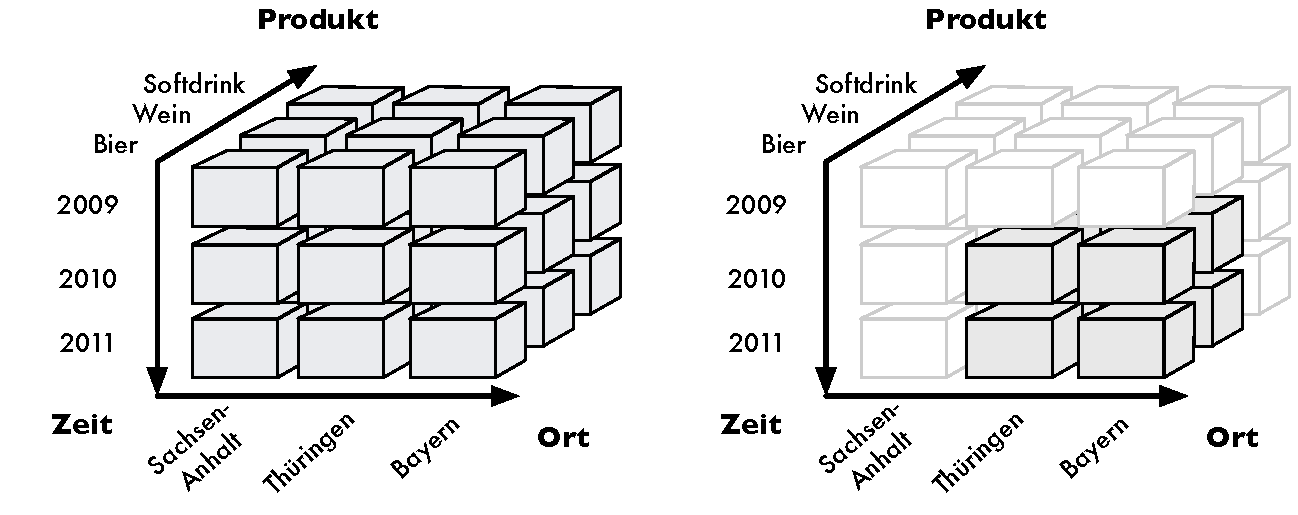
\includegraphics[width=.95\textwidth]{fig6/OLAP-Dice.pdf}
        \end{center}
        %Abbildung Slice
        
        \end{frame}
        
%-----------------------------------------------------------------------

\begin{frame}
    \frametitle{Umsetzung von OLAP-Operationen}

    \textbf{SQL}

    \begin{itemize}
        \item Star-Joins: Verbund der Faktentabelle mit den Dimensionstabellen, Gruppierung + Aggregation (siehe Teil III)
    \end{itemize}

    \textbf{Python + Pandas}

    \begin{itemize}
        \item \texttt{transpose}
        \item \texttt{groupby}, \texttt{pivot\_table}, \texttt{swaplevel}, \texttt{loc} + Indexierung
    \end{itemize}

\end{frame}  


\begin{frame}[fragile]
  \frametitle{Pandas: Pivot-Operationen}

  \begin{itemize}
    \item Daten umorganisieren (reshaping)
      \item \code{transpose}: Zeilen in Spalten umwandeln
    \end{itemize}

\begin{minted}{python}
df = pd.DataFrame({'A': [1, 2, 3, 4], 
                  'B': [10, 20, 30, 40],
                  'C': [100, 200, 300, 400]},
                  columns = ['A', 'B', 'C'])
df.transpose()
\end{minted}

{\small
\begin{center}
  \begin{tabular}{r|c|c|c|c|}
    \cline{2-5}
  & \textbf{0} & \textbf{1} & \textbf{2} & \textbf{3} \\
  \hline
  \textbf{A} &  1 & 2 & 3 & 4 \\
  \textbf{B} & 10 & 20 & 30 & 40 \\
  \textbf{C} & 100 & 200 & 300 & 400 \\
  \hline
  \end{tabular}
  \end{center}
  }
\end{frame}

\begin{frame}[fragile]
  \frametitle{Pandas: Pivot-Operationen /2}

  \begin{itemize}
      \item \code{pivot}: Konstruktion einer Pivot-Tabelle
      \begin{itemize}
      % \item zusätzlich angeben, welche Spalten im Ergebnis aufgenommen werden sollen
      \item benutzt \code{unique}-Werte der gegebenen Spalte
      \item keine Aggregationen
    \end{itemize}
    \item allgemeinere Form \code{pivot\_table}
    \end{itemize}

\end{frame}

\begin{frame}[fragile]
  \frametitle{Pandas: Pivot-Operationen /3}

  Tabelle \texttt{verkauf}

  \begin{center}
    \begin{tabular}{|c|c|c|}
    \hline
    \rowcolor{Gray} Bundesland & Jahr & Verkäufe \\
    \hline \hline
Thüringen      & 2019 &  100 \\
Thüringen      & 2020 & 105 \\
Sachsen        & 2019 & 141 \\
Sachsen        & 2020 & 143 \\
Sachsen-Anhalt & 2019 &  88 \\
Sachsen-Anhalt & 2020 &  94 \\
\hline
    \end{tabular}
  \end{center}
\end{frame}

\begin{frame}[fragile]
  \frametitle{Pandas: Pivot-Operationen /4}

  \begin{itemize}
\item Attribut \emph{Bundesland} wird ,,Index'', Attribut \emph{Verkäufe} wird aggregiert (hier summiert) 
  \end{itemize}

\begin{minted}{python}
verkauf.pivot_table(index=['Bundesland'], aggfunc='sum')
\end{minted}

\begin{center}
  \begin{tabular}{|c||c|}
  \hline
  \rowcolor{Gray}  & Verkäufe \\
  \rowcolor{Gray} Bundesland & \\
  \hline \hline
Sachsen        & 284 \\
Sachsen-Anhalt &  182 \\
Thüringen      &  205 \\
\hline 
  \end{tabular}
\end{center}

\end{frame}

\begin{frame}[fragile]
  \frametitle{Pandas: Pivot-Operationen /5}

  \begin{itemize}
\item mehrere Attribute können als Index dienen $\leadsto$ mehrdimensional
  \end{itemize}

\begin{minted}{python}
verkauf.pivot_table(index=['Bundesland', 'Jahr'], aggfunc='sum')
\end{minted}

{\small
\begin{center}
  \begin{tabular}{|c|c||c|}
  \hline
  \rowcolor{Gray}  & & Verkäufe \\
  \rowcolor{Gray} Bundesland & Jahr & \\
  \hline \hline
Sachsen        & 2019 & 141 \\
               & 2020 & 143 \\
Sachsen-Anhalt &  2019 & 88 \\
               & 2020 & 94 \\
Thüringen      &  2019 & 100 \\
               & 2020 & 105 \\
\hline 
  \end{tabular}
\end{center}
}

\end{frame}

\begin{frame}[fragile]
  \frametitle{Pandas: Gruppierung}

  \begin{itemize}
\item Gruppierung mit Aggregation ähnlich zu SQL
  \end{itemize}

\begin{minted}{python}
verkauf.groupby(['Bundesland', 'Jahr'])['Verkäufe'].sum()
\end{minted}

{\small
\begin{center}
  \begin{tabular}{|c|c||c|}
  \hline
  \rowcolor{Gray}  & &  \\
  \rowcolor{Gray} Bundesland & Jahr & \\
  \hline \hline
Sachsen        & 2019 & 141 \\
               & 2020 & 143 \\
Sachsen-Anhalt &  2019 & 88 \\
               & 2020 & 94 \\
Thüringen      &  2019 & 100 \\
               & 2020 & 105 \\
\hline 
  \end{tabular}
\end{center}
}
\end{frame}

\begin{frame}
        \frametitle{Zusammenfassung}
        
        \begin{itemize}
            \item In-Database-Analytics 
            \item Data Warehouse als Analyseplattform mit konsolidiertem und bereinigten Datenbestand
            \item Multidimensionales Datenmodell: Würfel, Kennzahlen, Dimensionen
            \item OLAP: konzeptionell, SQL, Python
        \end{itemize}
\end{frame}